\section{Marco conceptual}
\label{sec:marco_conceptual}
En esta sección se presentan conceptos y bases teóricas respecto a la temática que conduce el desarrollo de este trabajo, el cual tiene relación con el uso de interfaces no tradicionales, específicamente con una interfaz operada con el cuerpo. Además, se indaga sobre ciertas definiciones para establecer lo que se pretende medir en este estudio, lo que involucra la experiencia de usuario y métricas de rendimiento en la realización de tareas. Finalmente, se introducen las preguntas de investigación que guían el desarrollo de este trabajo.

\subsection{Recuperación de Información Humano Computador}
\label{subsec:HCIR}
La Recuperación de Información Humano Computador\footnote{Traducción libre.} (HCIR, por sus iniciales en inglés de \ingles{Human Computer Information Retrieval}) es el estudio de los métodos que integran la inteligencia humana y la búsqueda algorítmica para ayudar a la gente a mejorar la búsqueda, exploración y aprendizaje de información \parencite{marchionini2006}. Dentro de esta área interactúan otras disciplinas, como la recuperación de información, llamada en inglés \ingles{Information Retrieval} (IR), la que está enfocada principalmente en proveer a los usuarios un fácil acceso a la información de su interés trabajando con la representación, almacenamiento, organización y acceso a objetos de información como documentos, páginas \ingles{web}, catálogos en línea y objetos multimedia \parencite{ricardo2011modern} y la búsqueda de información, llamada en inglés \ingles{Information Seeking} (IS) que se entiende como un proceso más orientado al usuario y abierto que IR. En IS, no se sabe si existe una respuesta a la consulta del usuario, por lo que el proceso de búsqueda puede proporcionar el aprendizaje necesario para satisfacer su necesidad de información \parencite{ricardo2011modern}.

La búsqueda de información es un campo de la investigación que relaciona el desarrollo del área de las tecnologías y ciencias de la computación con la psicología y ciencias sociales en el procesamiento de la información, en donde el usuario toma un papel activo por medio de interacciones explicitas e implícitas con la información \parencite{carroll1997human}. Es una disciplina que contempla tanto al sistema como al usuario, así como la relación que se establece a través del comportamiento del usuario y sus experiencias \parencite{kelly2009methods}.

\subsection{Rendimiento}
\label{subsec:rendimiento}
En el contexto de la recuperación de información se definen \ingles{precision} y \ingles{recall} en función de un conjunto de documentos relevantes y un conjunto de documentos recuperados \parencite{powers2011evaluation}, las cuales se explican a continuación.  

\begin{description}
	\item [\ingles{Precision}] Métrica que mide la razón de documentos relevantes recuperados con 
respecto al total de documentos recuperados. Representado en la \eq{eq:precision}, el resultado de esta métrica es un valor continuo entre 0 y 1, mientras más cercano a 1, mayor fue su precisión al encontrar los documentos relevantes.

	\begin{equation}
	Precision = \frac{\big[\big\{documentos \ relevantes\big\} \cap \big\{documentos \ recuperados\big\}\big]}{\big\{documentos \ recuperados\big\}}
	\label{eq:precision}
	\end{equation}

	\item [\ingles{Recall}] Métrica que mide la razón de documentos relevantes recuperados con 
respecto al total de documentos relevantes. Representado en la \eq{eq:recall}, el resultado de esta métrica es un valor continuo entre 0 y 1, mientras más cercano a 1, mayor fue la recuperación de documentos en base al total del universo disponible.

	\begin{equation}
	Recall = \frac{\big[\big\{documentos \ relevantes\big\} \cap \big\{documentos \ recuperados\big\}\big]}{\big\{documentos \ relevantes\big\}}
	\label{eq:recall}
	\end{equation}

	\item [\ingles{F1}] Métrica que considera los valores de \ingles{precision} y \ingles{recall} en un promedio ponderado. Representado en la \eq{eq:F1}, el resultado de esta métrica es un valor continuo entre 0 y 1, en que un valor cercano a uno permite identificar a los estudiantes con una recuperación de documentos proporcional a su precisión respecto a la relevancia de estos.  

	\begin{equation}
	F1 = \frac{2 \cdot Precision\cdot Recall}{Precision+ Recall}
	\label{eq:F1}
	\end{equation}
 
\end{description}

%\begin{equation}
%	Precision = \frac{TP}{TP+ FP}
%\end{equation}
%\begin{equation}
%	Recall = \frac{TP}{TP+ FN}
%\end{equation}
\subsection{Alfabetización informacional}
\label{subsec:alfabetizacion}
La alfabetización informacional (conocida en inglés como \ingles{information literacy}) es definida como “el grupo de habilidades en las que se requiere reconocer cuándo la información es necesaria y tener la habilidad de encontrar, evaluar y usar efectivamente dicha información necesaria” \footnote{\traduccionlibre} \parencite[p.~2]{american2000information}. Es un campo que cubre varias áreas, entre las que se destaca la alfabetización digital, las habilidades de uso de bibliotecas, la ética informacional, la lectura crítica, el pensamiento crítico, los derechos de autor, la seguridad y privacidad, entre otras. A través del estudio de estas áreas como factores que influyen a la alfabetización informacional se puede obtener una visión clara de cómo los estudiantes llevan a cabo sus tareas de obtención y selección de información.

\subsection{Competencias de investigación en línea}
\label{subsec:competencias}
Se definen las competencias de investigación (\ingles{inquiry skills}, por su nombre en inglés) como “las habilidades para explorar preguntas, para poder reunir, interpretar y sintetizar diferentes tipos de información y datos, además de desarrollar y compartir una explicación para responder preguntas dadas” \footnote{\traduccionlibre} \parencite[p.~13]{national2000inquiry}. En base a este concepto nacen las competencias de investigación en línea (\ingles{online inquiry skills}, por su nombre en inglés), que son una instancia específica de las competencias de investigación, pero aplicada sobre información disponible en línea \parencite{quintana2005framework}.

Las competencias de investigación en línea involucran una serie de actividades cognitivas, como generar una pregunta de investigación, buscar información relevante en colecciones digitales, evaluar y seleccionar la información encontrada, e integrar coherentemente la información seleccionada para responder la pregunta original \parencite{eisenberg1990information}.

\subsection{Aprendizaje automático}
El aprendizaje automático (\ingles{machine learning}, por su nombre en inglés) es un área de la Inteligencia Artificial enfocada al desarrollo de algoritmos capaces de generalizar comportamientos, a partir de información no estructurada suministrada en forma de ejemplos, de manera que posean la capacidad de adaptarse en base a experiencia adquirida y no deban ser reprogramados. Los diversos algoritmos de esta rama se diferencian en su forma de llevar a cabo el aprendizaje, algunos de estos son:

\begin{description}
\item [Aprendizaje supervisado] Se realiza mediante un entrenamiento controlado por un agente externo (supervisor, maestro), que determina la respuesta que se debería generar a partir de una entrada determinada. El supervisor controla la salida y en caso de que esta no coincida con la deseada se modifican los parámetros usados, con el fin de conseguir que la salida obtenida se aproxime a la deseada.

\item [Aprendizaje no supervisado] Se realiza mediante un entrenamiento sin conocimiento a priori de la salida deseada, es decir, solo son conocidas las entradas, por lo tanto, el aprendizaje se basa en el grado de familiaridad o similitud entre la información que presenta una entrada y la información recolectada por entradas anteriores.
\end{description}

En cuanto al aprendizaje supervisado, uno de los problemas que intenta solucionar es la clasificación, cuya definición en este contexto corresponde al problema de identificar a qué categoría pertenece una nueva observación. 

Un clasificador se define como cualquier algoritmo que resuelva el problema de clasificación. Para ello, este tipo de algoritmo necesita ser entrenado con un conjunto de observaciones que ya estén etiquetadas en una categoría, de forma que pueda corregir su aprendizaje. Las observaciones son representadas a través de un conjunto de propiedades que permiten determinar a qué categoría pertenece. Por su parte, las propiedades pueden ser de tipo categórico (por ejemplo el tipo de sangre), ordinal (“grande”, “medio”, “pequeño”), valores enteros o reales o incluso utilizando la diferencia y similitud entre la observación actual y las observaciones previas. Como consecuencia del entrenamiento, se consigue un modelo del clasificador capaz de asignar observaciones desconocidas a una categoría conocida específica, solo sabiendo sus propiedades.

La terminología usada en esta área, suele llamar a las observaciones “instancias”, “ejemplos” o “sujetos”, a las propiedades “características” o “atributos”, a las categorías “clases”, al conjunto de observaciones “conjunto de entrada” y al conjunto de observaciones usadas en el entrenamiento “conjunto de entrenamiento”. Debido a las características de este proyecto, se utilizan técnicas de aprendizaje automático supervisado.

\subsection{Técnicas de minería de datos}
\label{subsec:tecnicas-mineria}
A continuación se presentan algunos de los modelos y algoritmos de minería de datos utilizados para extraer conocimiento desde los datos. Estos algoritmos son genéricos, pudiendo existir variantes de cada uno, ya que se van adaptando, combinando o incluyendo mejoras dependiendo del tipo de problema en estudio. 

\begin{itemize}
\item \textbf{\textit{K-Nearest Neighboor} (KNN)}: El algoritmo del K vecino más cercano o KNN es un de los algoritmos más simple. Este algoritmo no requiere de ningún parámetro fuera del número de vecinos a considerar. En pocas palabras, el algoritmo puede resumirse en que ``reúne los K vecinos más cercanos y los hace votar, la clase con más vecinos gana, mientras que más vecinos consideramos, menos la tasa de error''[22]. Dicha cercanía, generalmente se mide en base a alguna distancia, por lo que se pueden obtener distintos resultados dependiendo de la distancia escogida, pues diferentes métricas definirán diferentes regiones [26]. Su esquema general se propone en la siguiente Figura.

% TODO: insertar figura KDD


\item \textbf{Na\"ive Bayes}: En general los algoritmos de clasificación que utilizan el aprendizaje bayesiano resultan complejos en el sentido de la cantidad de parámetros. Sin embargo, el método de na\"ive bayes convierte dicha complejidad en una simpleza factible, “debido a que hace un supuesto de independencia con-
dicional que reduce el número de parámetros a estimar, cuando se modela P(x|y)” [76]. De forma cuantitativa, si la variable a predecir tiene dos valores pasa de estimar 2 (2n − 1) parámetros a 2n. La utilidad de los algoritmos de aprendizaje bayesiano es que “da una medida probabilística de la importancia de esas variables en el problema, y, por lo tanto, una probabilidad explícita de las hipótesis que se formulan” [68].

\item \textbf{Árboles de decisión}: Los árboles de decisión son modelos que usualmente se representan en forma de grafos. Es ``un modelo predictivo que puede ser usado para representar tanto modelos regresivos como aquellos de clasificación, se refiere a un modelo jerárquico de decisiones y sus consecuencias'' [33]. Dentro de un esquema general, el árbol de decisión consiste en un grafo donde existe un nodo único o padre, el cual, contiene las instancias a contemplar en el modelo. Un ejemplo de este tipo de modelos es el LADTree, el cual es un tipo de árbol de decisión que itera sobre el ADTree, que es un árbol que en vez de establecer criterios y dividir la muestra, asigna una puntuación a las categorías relevantes de determinadas variables.



\item \textbf{Máquina vectorial de soporte (SVM)}: A diferencia de los algoritmos anteriores, la máquina de soporte vectorial, o bien, \ingles{Support Vector Machines}, utilizan planos complejos para encontrar la mejor división de las instancias que permita clasificarlas de manera óptima. Cuya formulación es un problema de minimización cuadrática con un número de variables igual al número de casos de entrenamiento.

\item \textbf{Redes neuronales}: Una red neuronal artificial (o denominada simplemente red neuronal, o ANN) ``consiste en procesar elementos (llamados neuronas)''

\item \textbf{Regresión}: La regresión, consiste en ``\textit{el estudio de la dependencia de la variable dependiente, respecto a una o más variables, con el objetivo de estimar y/o predecir la media o valor promedio poblacional de la primera en términos de los valores conocidos o fijos (en muestras repetidas) de las últimas}'' [19]. Por lo que este modelo sirve para predecir y clasificar, donde su uso típico es el de predecir la demanda o el inventario futuro de una empresa. En el caso de la clasificación, la regresión que se utiliza comúnmente no resulta muy efectiva, puesto que la variable a predecir posee una connotación nominal, sin embargado, existe un tipo de regresión que se encarga de predecir variables nominales y se denomina regresión logística.


\item \textbf{Multiclasificadores}:
\end{itemize}

\subsubsection*{Árboles de decisión}

\begin{figure}[H]
	\centering
	\newdimen\nodeDist
\nodeDist=35mm

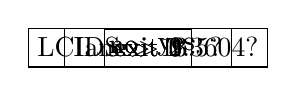
\begin{tikzpicture}[
    node/.style={%
      draw,
      rectangle,
    },
  ]

    \node [node] (A) {IDS $>$ 13.5?};
    \path (A) ++(-135:\nodeDist) node [node] (B) {exit 1};
    \path (A) ++(-45:\nodeDist) node [node] (C) {LCIanx $>$ 0.3604?};
    \path (C) ++(-135:\nodeDist) node [node] (D) {exit 2};
    \path (C) ++(-45:\nodeDist) node [node] (E) {exit 3};

    \draw (A) -- (B) node [left,pos=0.25] {no}(A);
    \draw (A) -- (C) node [right,pos=0.25] {yes}(A);
    \draw (C) -- (D) node [left,pos=0.25] {no}(A);
    \draw (C) -- (E) node [right,pos=0.25] {yes}(A);
\end{tikzpicture}
	\captionsource{Árbol de decisión}{\fuentePropia}
	\label{fig:decision-tree}
\end{figure}


\subsubsection*{Máquinas de vectores de soporte (SVM)}
Las máquinas de vectores de soporte o SVM (del inglés \ingles{Support Vector Machine}) son un conjunto de algoritmos de aprendizaje supervisado que se enfocan en resolver problemas de clasificación, regresión y agrupamiento. La SVM destinada para clasificación, es un clasificador lineal binario que busca encontrar un hiperplano que separe de forma óptima un conjunto de datos, maximizando la distancia entre las dos clases.


\begin{figure}[H]
	\centering
	\begin{tikzpicture}[&gt;=stealth']
  % Draw axes
  \draw [&lt;-&gt;,thick] (0,5) node (yaxis) [above] {$y$}
        |- (5,0) node (xaxis) [right] {$x$};
  % draw line
  \draw (0,-1) -- (5,4); % y=x-1
  \draw[dashed] (-1,0) -- (4,5); % y=x+1
  \draw[dashed] (2,-1) -- (6,3); % y=x-3
  % \draw labels
  \draw (3.5,3) node[rotate=45,font=\small] 
        {$\mathbf{w}\cdot \mathbf{x} + b = 0$};
  \draw (2.5,4) node[rotate=45,font=\small] 
        {$\mathbf{w}\cdot \mathbf{x} + b > 1$};
  \draw (4.5,2) node[rotate=45,font=\small] 
        {$\mathbf{w}\cdot \mathbf{x} + b < -1$};
  % draw distance
  \draw[dotted] (4,5) -- (6,3);
  \draw (5.25,4.25) node[rotate=-45] {$\frac{2}{\Vert \mathbf{w} \Vert}$};
  \draw[dotted] (0,0) -- (0.5,-0.5);
  \draw (0,-0.5) node[rotate=-45] {$\frac{b}{\Vert \mathbf{w} \Vert}$};
  \draw[-&gt;] (2,1) -- (1.5,1.5);
  \draw (1.85,1.35) node[rotate=-45] {$\mathbf{w}$};
  % draw negative dots
  \fill[red] (0.5,1.5) circle (3pt);
  \fill[red]   (1.5,2.5)   circle (3pt);
  \fill[black] (1,2.5)     circle (3pt);
  \fill[black] (0.75,2)    circle (3pt);
  \fill[black] (0.6,1.9)   circle (3pt);
  \fill[black] (0.77, 2.5) circle (3pt);
  \fill[black] (1.5,3)     circle (3pt);
  \fill[black] (1.3,3.3)   circle (3pt);
  \fill[black] (0.6,3.2)   circle (3pt);
  % draw positive dots
  \draw[red,thick] (4,1)     circle (3pt); 
  \draw[red,thick] (3.3,.3)  circle (3pt); 
  \draw[black]     (4.5,1.2) circle (3pt); 
  \draw[black]     (4.5,.5)  circle (3pt); 
  \draw[black]     (3.9,.7)  circle (3pt); 
  \draw[black]     (5,1)     circle (3pt); 
  \draw[black]     (3.5,.2)  circle (3pt); 
  \draw[black]     (4,.3)    circle (3pt); 
\end{tikzpicture}
	\captionsource{SVM}{\fuentePropia}
	\label{fig:svm}
\end{figure}

\subsubsection*{Perceptrón}

\begin{figure}[H]
	\centering
	% Multilayer perceptron
\usetikzlibrary{positioning}

\tikzstyle{inputNode}=[draw,circle,minimum size=10pt,inner sep=0pt]
\tikzstyle{stateTransition}=[-stealth, thick]

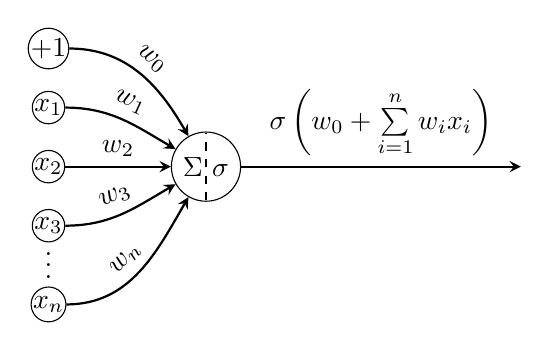
\begin{tikzpicture}
    \node[draw,circle,minimum size=25pt,inner sep=0pt] (x) at (0,0) {$\Sigma$ $\sigma$};

    \node[inputNode] (x0) at (-2, 1.5) {$\tiny +1$};
    \node[inputNode] (x1) at (-2, 0.75) {$\tiny x_1$};
    \node[inputNode] (x2) at (-2, 0) {$\tiny x_2$};
    \node[inputNode] (x3) at (-2, -0.75) {$\tiny x_3$};
    \node[inputNode] (xn) at (-2, -1.75) {$\tiny x_n$};

    \draw[stateTransition] (x0) to[out=0,in=120] node [midway, sloped, above] {$w_0$} (x);
    \draw[stateTransition] (x1) to[out=0,in=150] node [midway, sloped, above] {$w_1$} (x);
    \draw[stateTransition] (x2) to[out=0,in=180] node [midway, sloped, above] {$w_2$} (x);
    \draw[stateTransition] (x3) to[out=0,in=210] node [midway, sloped, above] {$w_3$} (x);
    \draw[stateTransition] (xn) to[out=0,in=240] node [midway, sloped, above] {$w_n$} (x);
    \draw[stateTransition] (x) -- (4,0) node [midway,above] {$\sigma\left(w_0 + \sum\limits_{i=1}^{n}{w_ix_i}\right)$};
    \draw[dashed] (0,-0.43) -- (0,0.43);
    \node (dots) at (-2, -1.15) {$\vdots$};
    
\end{tikzpicture}

	\captionsource{Perceptrón}{\fuentePropia}
	\label{fig:perceptron}
\end{figure}

\begin{equation}
 \pmb{\mu_1} = \begin{bmatrix}0\\0\\...\\0\end{bmatrix}
\end{equation}

\subsubsection*{Perceptrón multicapa}

\begin{figure}[H]
	\centering
	% Multilayer perceptron
\usetikzlibrary{positioning}

\tikzstyle{inputNode}=[draw,circle,minimum size=10pt,inner sep=0pt]
\tikzstyle{stateTransition}=[-stealth, thick]

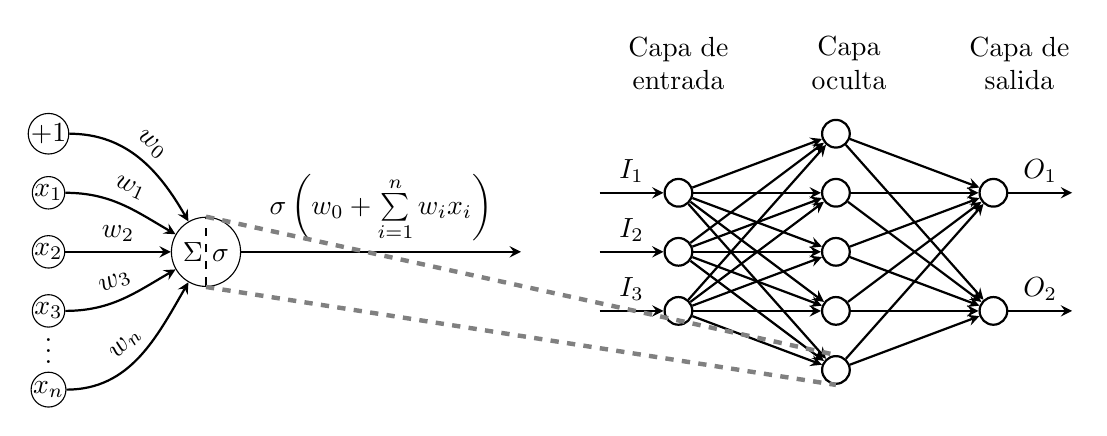
\begin{tikzpicture}
    \node[draw,circle,minimum size=25pt,inner sep=0pt] (x) at (0,0) {$\Sigma$ $\sigma$};

    \node[inputNode] (x0) at (-2, 1.5) {$\tiny +1$};
    \node[inputNode] (x1) at (-2, 0.75) {$\tiny x_1$};
    \node[inputNode] (x2) at (-2, 0) {$\tiny x_2$};
    \node[inputNode] (x3) at (-2, -0.75) {$\tiny x_3$};
    \node[inputNode] (xn) at (-2, -1.75) {$\tiny x_n$};

    \draw[stateTransition] (x0) to[out=0,in=120] node [midway, sloped, above] {$w_0$} (x);
    \draw[stateTransition] (x1) to[out=0,in=150] node [midway, sloped, above] {$w_1$} (x);
    \draw[stateTransition] (x2) to[out=0,in=180] node [midway, sloped, above] {$w_2$} (x);
    \draw[stateTransition] (x3) to[out=0,in=210] node [midway, sloped, above] {$w_3$} (x);
    \draw[stateTransition] (xn) to[out=0,in=240] node [midway, sloped, above] {$w_n$} (x);
    \draw[stateTransition] (x) -- (4,0) node [midway,above] {$\sigma\left(w_0 + \sum\limits_{i=1}^{n}{w_ix_i}\right)$};
    \draw[dashed] (0,-0.43) -- (0,0.43);
    \node (dots) at (-2, -1.15) {$\vdots$};
    \node[inputNode, thick] (i1) at (6, 0.75) {};
    \node[inputNode, thick] (i2) at (6, 0) {};
    \node[inputNode, thick] (i3) at (6, -0.75) {};
    
    \node[inputNode, thick] (h1) at (8, 1.5) {};
    \node[inputNode, thick] (h2) at (8, 0.75) {};
    \node[inputNode, thick] (h3) at (8, 0) {};
    \node[inputNode, thick] (h4) at (8, -0.75) {};
    \node[inputNode, thick] (h5) at (8, -1.5) {};
    
    \node[inputNode, thick] (o1) at (10, 0.75) {};
    \node[inputNode, thick] (o2) at (10, -0.75) {};
    
    \draw[stateTransition] (5, 0.75) -- node[above] {$I_1$} (i1);
    \draw[stateTransition] (5, 0) -- node[above] {$I_2$} (i2);
    \draw[stateTransition] (5, -0.75) -- node[above] {$I_3$} (i3);
    
    \draw[stateTransition] (i1) -- (h1);
    \draw[stateTransition] (i1) -- (h2);
    \draw[stateTransition] (i1) -- (h3);
    \draw[stateTransition] (i1) -- (h4);
    \draw[stateTransition] (i1) -- (h5);
    \draw[stateTransition] (i2) -- (h1);
    \draw[stateTransition] (i2) -- (h2);
    \draw[stateTransition] (i2) -- (h3);
    \draw[stateTransition] (i2) -- (h4);
    \draw[stateTransition] (i2) -- (h5);
    \draw[stateTransition] (i3) -- (h1);
    \draw[stateTransition] (i3) -- (h2);
    \draw[stateTransition] (i3) -- (h3);
    \draw[stateTransition] (i3) -- (h4);
    \draw[stateTransition] (i3) -- (h5);
    
    \draw[stateTransition] (h1) -- (o1);
    \draw[stateTransition] (h1) -- (o2);
    \draw[stateTransition] (h2) -- (o1);
    \draw[stateTransition] (h2) -- (o2);
    \draw[stateTransition] (h3) -- (o1);
    \draw[stateTransition] (h3) -- (o2);
    \draw[stateTransition] (h4) -- (o1);
    \draw[stateTransition] (h4) -- (o2);
    \draw[stateTransition] (h5) -- (o1);
    \draw[stateTransition] (h5) -- (o2);
    
    %Input layer
    \node[above=of i1, align=center] (l1) {Capa de \\ entrada};
    %Hidden Layer
    \node[right=2.3em of l1, align=center] (l2) {Capa \\ oculta};
    %Output Layer
    \node[right=2.3em of l2, align=center] (l3) {Capa de \\ salida};
    
    \draw[stateTransition] (o1) -- node[above] {$O_1$} (11, 0.75);
    \draw[stateTransition] (o2) -- node[above] {$O_2$} (11, -0.75);
    
    \path[dashed, double, ultra thick, gray] (x.north) edge[bend left=0] (h5.north);
    \path[dashed, double, ultra thick, gray] (x.south) edge[bend right=0] (h5.south);
\end{tikzpicture}

	\captionsource{Perceptrón multicapa}{\fuentePropia}
	\label{fig:multilayer-perceptron}
\end{figure}

\subsubsection*{Na\"ive Bayes}
El clasificador Na\"ive Bayes, también conocido como clasificador bayesiano, es un clasificador probabilístico basado en el teorema de Bayes descrito en la \eq{eq:naive-bayes}, donde $P(A|B)$ es la probabilidad de la hipótesis.

\begin{equation}
 P(A|B) = \frac{P(A) \cdot P(B|A)}{P(B)}
 \label{eq:naive-bayes}
\end{equation}


\subsection{Técnicas de reforzamiento}


\begin{figure}[H]
	\centering
	\tikzstyle{block} = [rectangle, draw, 
    text width=8em, text centered, rounded corners, minimum height=4em]
    
\tikzstyle{line} = [draw, -latex]

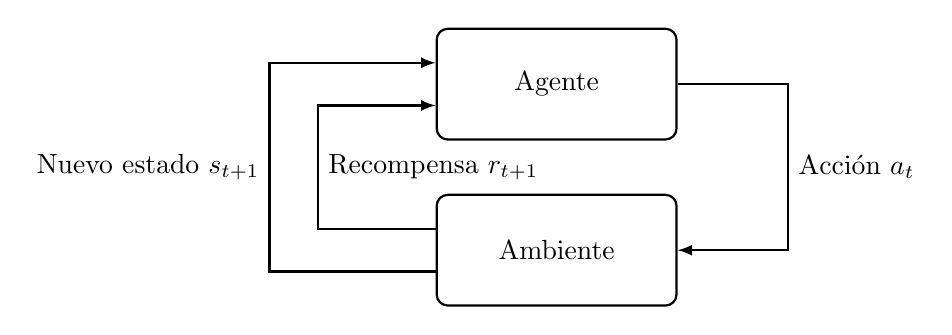
\begin{tikzpicture}[node distance = 6em, auto, thick]
    \node [block] (Agent) {Agente};
    \node [block, below of=Agent] (Environment) {Ambiente};
    
     \path [line] (Agent.0) --++ (4em,0em) |- node [near start]{Acción $a_t$} (Environment.0);
     \path [line] (Environment.190) --++ (-6em,0em) |- node [near start] {Nuevo estado  $s_{t+1}$} (Agent.170);
     \path [line] (Environment.170) --++ (-4.25em,0em) |- node [near start, right] {Recompensa $r_{t+1}$} (Agent.190);
\end{tikzpicture}
	\captionsource{Aprendizaje por reforzamiento}{\fuentePropia}
	\label{fig:decision-tree}
\end{figure}


\subsection{Comparación entre los principales algoritmos de aprendizaje automático}
A continuación se describen brevemente los modelos básicos con sus ventajas y desventajas.

\begin{itemize}
\item \textbf{SVM (Support Vector Machines)}: Usando las funciones Kernel se pueden incluir distintos grados de no linealidad y de esta manera, flexibilizar el modelo.

La desventaja de este modelo es que el resultado de la clasifícación es puramente dicotómico y no hay probabilidad de pertenencia, además, no se tiene una idea clara de explicación dada la complejidad del modelo en sí.

\item \textbf{K- vecino más cercano (\textit{K-Nearest neighbor})}: La ventaja es que los vecinos pueden dar una explicación de los resultados de clasificación. La desventaja de este modelo es que requiere definir una métrica que mida la distancia entre los datos, puesto que no es clara como definir dicha métrica.

\item \textbf{Árboles de decisión}: La desventaja de este modelo está en que las variables continuas o numéricas son implícitamente discretizadas en el proceso de separación, perdiendo información en el camino. No obstante, previo al análisis anterior, los árboles son tolerantes al ruido, a los atributos no significativos y a los valores faltantes; son escalables a grandes volúmenes.

Dentro de sus desventajas están la de su imprecisión y su debilidad en el sentido de que dos muestras distintas sobre la misma distribución pueden llevar a dos árboles muy diferentes. La ventaja es que establece una explicación clara acerca de la predicción.

\item \textbf{Regresión lineal}: Este modelo es flexible por el hecho de que se pueden incluir términos de interacción, es decir, productos que hagan el modelo no lineal. La desventaja es que no posee alto grado como las redes neuronales ya que la alta flexibilidad conlleva un alto riesgo de sobreajuste u \ingles{overfitting}, lo que reduce el \ingles{accuracy}.

\end{itemize}


\subsection{Minería de datos educacional}
La minería de datos utiliza una combinación de bases de conocimientos explícita, conocimientos analíticos complejos y conocimiento de campo para descubrir las tendencias y los patrones ocultos, estas tendencias y patrones forman la base de los modelos predictivos que permiten a los analistas realizar nuevas observaciones de los datos existentes \parencite{luan2002data}. La gran cantidad de información generada hoy en día por los estudiantes permite que la minería de datos obtenga datos relevantes y, a través de métodos estadísticos y otras herramientas relacione la información para conocer si el proceso de enseñanza aprendizaje ha dado resultados positivos. 

\textcite[p.~9]{mining2012enhancing} define la minería de datos educacional (MDE, desde ahora en adelante) como “la teoría que desarrolla métodos, aplica técnicas estadísticas y de aprendizaje automático para analizar los datos recogidos durante el proceso de la enseñanza y aprendizaje”\footnote{\traduccionlibre}. Actualmente, los usos más generales que se le están dando a la MDE se enfocan en mejorar la estructura del conocimiento y determinar el apoyo pedagógico al estudiante.